

% Nastaven� �ablony FM TUL
% nastaveni prezentace
%\documentclass[draft]{beamer}
\documentclass[t]{beamer}

\usepackage[czech]{babel}

% FONTY

%\usepackage[cp1250]{inputenc} % pro win1250
\usepackage[T1]{fontenc}

\usepackage[utf8]{inputenc}
%\usepackage[IL2]{fontenc}

\usepackage{lmodern}

% XeLaTeX
%\usepackage{fontspec,lipsum}
%\defaultfontfeatures{Ligatures=TeX}
%\usepackage[small,sf,bf]{titlesec}
% 
%\setromanfont{Georgia}
%\setsansfont{Myriad Pro} %Tahoma}
%\setsansfont{Tahoma}
%\setsansfont{Arial}
%\setsansfont{Times New Roman}
%====

% bohu�el dal�� fonty nejsou pln� po�e�t�n�, tedy nejde bez obt��� kop�rovat z PDF

%\usepackage{times}
% \usepackage{avant}
% \usepackage{bookman}
% \usepackage{helvet}  %chyb� tu�n� �ez u strojov�ho p�sma
% \usepackage{newcent}
% \usepackage{palatino} 



%\usepackage[scaled]{uarial}
%\usepackage{helvet}


\usepackage{hyperref}

\mode<presentation>
{
  \definecolor{FM_TUL}{cmyk}{0,0.6,1,0}
  
  \useinnertheme{rectangles}
  
  % VN�J�� BAREVN� T�MA NADPIS�    
  \usecolortheme{whale}  
  
  % VNIT�N� BAREVN� T�MA V��T�, BLOK� ATD.  
  \usecolortheme{orchid}

  \setbeamercolor{titlelike}{parent=structure}
  \setbeamercolor{frametitle}{fg=black}
  \setbeamercolor{title}{fg=black}
  \setbeamercolor{item}{fg=FM_TUL} 
  \setbeamertemplate{navigation symbols}{} % potla�en� naviga�n�ch symbol�
  \setbeamercolor{block title}{fg=white,bg=FM_TUL} % p�edefinov�n� barvy z�kl. bloku
  \setbeamercolor{caption name}{fg=FM_TUL}
  
%  Nadpisy slid� tu�n� dokud nevy�e��m pou�it� font� tak, aby se dalo kop�rovat z pdf
%  \setbeamercolor{frametitle}{fg=FM_TUL}
  \setbeamertemplate{frametitle}
  {
    \textbf{\insertframetitle}
    \par
  }
  \setbeamercolor{bibliography entry author}{fg=black} % literatura �ern� a ne mod�e
  \setbeamercolor{bibliography entry title}{fg=black} % literatura �ern� a ne mod�e
  \setbeamercolor{bibliography entry journal}{fg=black} % literatura �ern� a ne mod�e
  \setbeamercolor{bibliography entry note}{fg=black} % literatura �ern� a ne mod�e
  
%Nefunguje  \setbeamercolor{tableofcontents}{fg=TUL_FM} % obsah TUL_FM a ne mod�e
}

%===============================================================================
% TITULN� STRANA
%===============================================================================
\setbeamertemplate{title page}{
\begin{flushleft}
   
\includegraphics[width=0.6\textwidth]{obr/logo-fm-cmyk-cz.pdf}
\end{flushleft} 
  %
\begin{center} 
  \setbeamercolor{postit}{fg=black,bg=FM_TUL}
%  \begin{beamercolorbox}[center,sep=2pt,wd=\textwidth,ht=3cm,dp=20pt]{postit}
 \begin{beamercolorbox}[center,sep=10pt,wd=\textwidth,ht=3.2cm,ignorebg]{postit}
            
      {\bf {\LARGE \inserttitle}}\\[16pt]
              
      \insertsubtitle
  \end{beamercolorbox}
%
  \vspace{10pt}
  {\bf \small \insertauthor {\color{FM_TUL} ~|} \insertdate}
%  \vspace{10pt}    
\end{center}
%
\vfill
\vskip0pt plus 1filll
{\color{FM_TUL} \hrule} 
%
\begin{center}
\vspace{-8pt}         
\TextTitulniStranaPodLinkou
\end{center}   
}
%===============================================================================
% Z�HLAV� KA�D�HO SLAJDU
%===============================================================================
\setbeamertemplate{headline}{
  \hspace{-3pt}
\includegraphics[width=0.3\textwidth]{obr/logo-fm-cmyk-cz.pdf}
}
%===============================================================================
\setbeamertemplate{footline}{

\includegraphics[width=\textwidth]{obr/FM_TUL_linka_piktogram_obd.pdf}

\vspace{-9.5pt}
~\hfill {\tiny\color{white} \insertframenumber\,/\,\inserttotalframenumber}\hspace{5pt}

\hspace{3pt} {\tiny \inserttitle {\color{FM_TUL} ~|} \insertdate }\hspace{3pt}
\vspace{3pt}
}
%===============================================================================
% �PRAVA BARVY TEXTU V OBSAHU 
%===============================================================================
\setbeamercolor{section in toc}{fg=black}
\setbeamercolor{subsection in toc}{fg=black}
\setbeamercolor{subsubsection in toc}{fg=black}
\setbeamercolor{button}{bg=FM_TUL}

%\definecolor{links}{HTML}{2A1B81}
\hypersetup{colorlinks,linkcolor=,urlcolor=FM_TUL}


\usepackage{palatino}
\usepackage{graphicx}
\usepackage{transparent}

\setbeamercovered{transparent=35}

\title[Editor konfiguračních souborů~Flow123d]{Editor konfiguračních souborů~Flow123d}
\subtitle{Diplomová práce}
\author[Bc. Tomáš Křížek]{Bc. Tomáš Křížek}
\institute[TUL]{Technická univerzita v Liberci}
\date{19.~dubna~2016}
\newcommand{\TextTitulniStranaPodLinkou}{\tiny
Studentská 2 {\color{FM_TUL} |} 461\,17 Liberec 2 {\color{FM_TUL} |} {tomas.krizek1@tul.cz} {\color{FM_TUL} |} 
\href{http://www.fm.tul.cz/}{www.fm.tul.cz}}

\begin{document}
%\setbeamertemplate{caption}{\insertcaption}


\begin{frame}
	\titlepage
\end{frame}

\begin{frame}
	\frametitle{Obsah}
	\begin{itemize}
		\item Problematika
		\item Motivace
		\item Zpracování konfiguračního souboru
		\item Validace
		\item Kontextová nápověda
		\item Grafické rozhraní
		\item Použité technologie
	\end{itemize}
\end{frame}


\begin{frame}[t]
	\frametitle{Problematika}
	\begin{block}{Simulátor Flow123d}
	\begin{itemize}[<+->]
		\item modelování procesů v horninovém prostředí
		\item pouze textové rozhraní
		\item výpočetně náročné $\rightarrow$ vzdálené spouštění
	\end{itemize}
	\end{block}
	
	\begin{block}{Konfigurační soubory}
	\begin{itemize}[<+->]
		\item definice úlohy
		\item rozsáhlé možnosti nastavení
		\item záznamy, pole, primitivní datové typy, abstraktní záznamy
	\end{itemize}
	\end{block}
\end{frame}

\begin{frame}[t]
	\frametitle{Motivace}
	\begin{block}{Chyby v konfiguračních souborech}
	\begin{itemize}[<+->]
		\item časově náročná detekce a odstranění
		\item uživatelsky nepřívětivé
	\end{itemize}
	\end{block}
	
	\begin{block}{Vytváření a upravování konfiguračních souborů}
	\begin{itemize}[<+->]
		\item běžné textové editory
		\item rozsáhlá referenční dokumentace formátu
	\end{itemize}
	\end{block}
	
	\onslide<5>{
	\vspace{0.5cm}
	$\Rightarrow$ \textit{specializovaný editor}
	}
\end{frame}

\begin{frame}[fragile]
	\frametitle{Zpracování konfiguračního souboru}
	\only<1>{
	\hspace*{-5pt}
\includegraphics[width=\textwidth]{../../img/data_structure_chain_1.pdf}\\
	}
	\only<2-5>{
	\hspace*{-5pt}
\includegraphics[width=\textwidth]{../../img/data_structure_chain_2.pdf}\\
	}
	\only<6-9>{
	\hspace*{-5pt}
\includegraphics[width=\textwidth]{../../img/data_structure_chain_3.pdf}\\
	}
	\only<10>{
	\hspace*{-5pt}
\includegraphics[width=\textwidth]{../../img/data_structure_chain_4.pdf}\\
	}
	\begin{minipage}[t]{0.45\textwidth}
	\begin{block}{Formát YAML}
	\begin{itemize}
		\item<3-> nahrazuje formát CON
		\item<4-> přehledná syntaxe
		\item<5-> návrh použití syntaxe pro zápis (abstraktní záznamy, reference)
		%\item<6-> vlastní implementace zpracování souboru
	\end{itemize}
	\end{block}
	\end{minipage}
	\hspace{5pt}
	\begin{minipage}[t]{0.45\textwidth}
	\begin{block}{Autokonverze}
	\begin{itemize}
		\item<7-> speciální zkrácený zápis polí či záznamů
		\item<8-> v praxi -- jiný datový typ, než se očekává
		\item<9-> libovolně vnořené $\rightarrow$ rekurzivní průchod datové struktury
	\end{itemize}
	\end{block}
	\end{minipage}
\end{frame}

\begin{frame}
	\frametitle{Validace}
	\begin{itemize}[<+->]
	\item včasné odhalení chyb
	\item přizpůsobí se verzi Flow123d
	\item upozornění na možné problémy
	\end{itemize}
	\only<1-3>{
		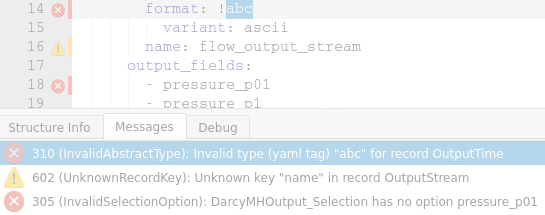
\includegraphics[width=\textwidth]{img/validation_pause.png}
	}
	\only<4->{
		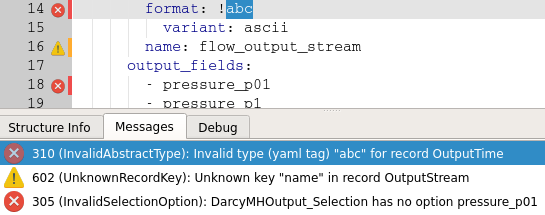
\includegraphics[width=\textwidth]{img/validation.png}
	}
\end{frame}


\begin{frame}
	\frametitle{Kontextová nápověda}
	\begin{itemize}[<+->]
	\item alternativa k rozsáhlé referenční dokumentaci
	\item zobrazuje relevantní dokumentaci k právě editované hodnotě (pozici)
	\item možnost navigace v rámci nápovědy
	\end{itemize}
	\only<1-3>{
		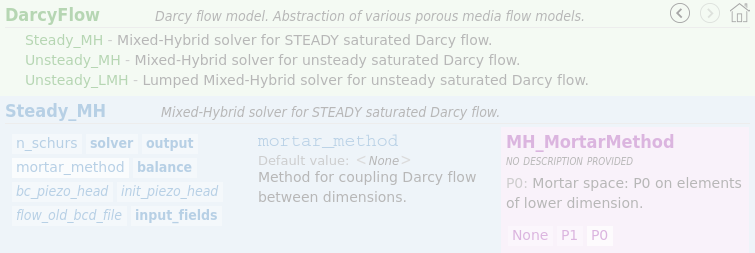
\includegraphics[width=\textwidth]{img/gui_doc_mortar_method_pause.png}
	}
	\only<4->{
		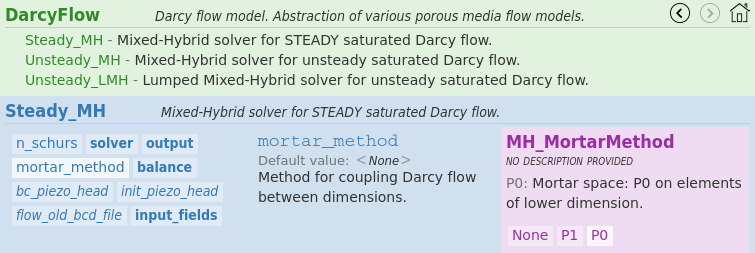
\includegraphics[width=\textwidth]{img/gui_doc_mortar_method.png}
	}
\end{frame}

\begin{frame}
	\frametitle{Grafické rozhraní aplikace}
	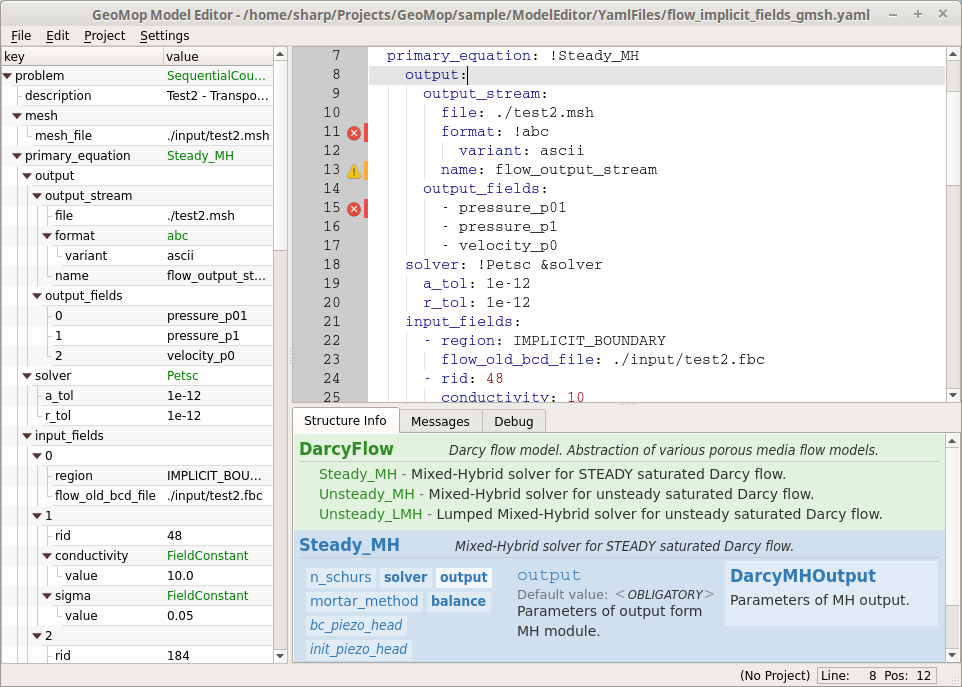
\includegraphics[height=7cm]{img/gui.png}
\end{frame}

\begin{frame}
	\frametitle{Použité technologie}
	\begin{itemize}[<+->]
	\item Python 3.4
	\item grafická knihovna PyQt 5
	\item knihovna pro textový editor QScintilla 2
	\item knihovna pro YAML -- PyYAML
	\item instalační balíčky pro Windows, Debian
	\end{itemize}
\end{frame}

\begin{frame}
	\frametitle{Shrnutí -- funkce editoru}
	\begin{itemize}[<+->]
	\item zpracování YAML
	\item autokonverze
	\item validace
	\item kontextová nápověda
	\item automatické doplňování textu
	\item vizualizace datové struktury
	\item přizpůsobí se verzi Flow123d
	\item multiplatformní aplikace (Windows XP a novější, Linux)
	\end{itemize}
\end{frame}

\begin{frame}{}{}
\begin{center}
\huge Děkuji za pozornost.
\end{center}
\end{frame}


\end{document}
